\documentclass[a4paper,12pt]{amsart}

\usetheme[progressbar=frametitle]{metropolis}
\metroset{block=fill}

\subtitle{NTIN071 Automata and Grammars}
\author{Jakub Bulín (KTIML MFF UK)}

\date{Spring 2025\\ 
    \vspace{1in} 
    \begin{flushleft}
        \it \footnotesize * Adapted from the Czech-lecture slides by Marta Vomlelová with gratitude. The translation, some modifications, and all errors are mine.
    \end{flushleft}
}

%% packages

\usepackage{amsmath}
\usepackage{amssymb}
\usepackage{amsthm}
\usepackage{cancel}
\usepackage{color}
\usepackage{colortbl}
\usepackage{forest}
\usepackage[utf8x]{inputenc}
\usepackage{multicol}
\usepackage{multirow}

%% colors
\definecolor{Gray}{gray}{0.9}

%% TikZ
\usepackage{tikz}
    \usetikzlibrary{
        automata,
        arrows,
        backgrounds,
        decorations.pathmorphing,
        fit,
        positioning,
        shapes,
        shapes.geometric,
        tikzmark
    } 
    \tikzset{>=stealth',shorten >=1pt,auto,node distance=2cm}
    \tikzset{initial text={}}
    \tikzset{elliptic state/.style={draw,ellipse}}

%% amsthm
\theoremstyle{plain}
    \newtheorem*{algorithm}{Algorithm}    
    \newtheorem*{observation}{Observation}
    \newtheorem*{proposition}{Proposition}

\theoremstyle{remark}
    \newtheorem*{exercise}{Exercise}
    \newtheorem*{remark}{Remark}

%% macros
\DeclareMathOperator{\RegE}{RegE}
\DeclareMathOperator{\RL}{RL}

% Just for Lecture 2
\newcommand{\x}{$\times$}
\newcommand{\nx}{\ }


\begin{document}

% \thispagestyle{empty}

\section*{NTIN071 A\&G: Tutorial 5 -- More regular expressions, TODO}

% after Lecture 5
% spring 2024

\medskip

% \noindent\emph{Solve 1a, 2abc, 3 (the rest is for practice).}

\medskip


\medskip\begin{problem}[Testing equivalence of regular expressions]

    \phantom{}

    \medskip

    \begin{enumerate}[(a)]\setlength\itemsep{12pt}
        \item Describe an algorithm to test equivalence of two regular expressions.
        \item Apply it to the following pair of regular expressions:
        $$
        (a + b)(a + b)^* \qquad\text{and}\qquad a(a + b)^* + b(a + b)^*
        $$
    \end{enumerate}
    
\end{problem}

    
\medskip\begin{problem}[Automaton to regex]
    
    Construct regular expressions for languages accepted by the following automata.

    \bigskip
    
    \begin{multicols}{2}
    
        \begin{enumerate}[(a)]\setlength\itemsep{12pt}
        
            \item 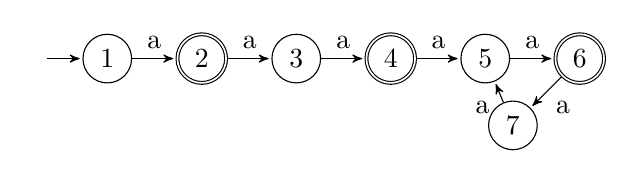
\begin{tikzpicture}[>=stealth',shorten >=1pt,auto,node distance=1.2cm]
                    \tikzset{every state/.style={minimum size=0.2cm}}
                        
                        \node[initial,state]  (a1)      {1};
                        \node[state,accepting] (b1)  [right of=a1]    {2};
                            \node[state] [right of=b1](c1)      {3};
                        \node[state,accepting] [right of=c1] (d1)      {4};
                        \node[state] (e1)  [right of=d1]    {5};
                        \node[state,accepting] (f1)  [right of=e1]    {6};
                        \node[state] (g1)  [below left of=f1]    {7};
                    \path[->]
                            (a1)  edge  node {a} (b1)
                            (b1)  edge  node {a} (c1)
                            (c1)  edge  node {a} (d1)
                            (d1)  edge  node {a} (e1)
                            (e1)  edge  node {a} (f1)
                            (f1)  edge  node {a} (g1)
                            (g1)  edge  node {a} (e1)
                            ;
            \end{tikzpicture}
            
            \item 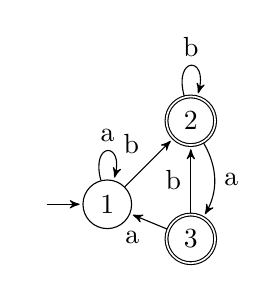
\begin{tikzpicture}[>=stealth',shorten >=1pt,auto,node distance=1.5cm]
                    \tikzset{every state/.style={minimum size=0.2cm}}
                        
                        \node[initial,state]  (a1)      {1};
                        \node[state,accepting] (b1)  [above right of=a1]    {2};
                            \node[state,accepting] [below of=b1](c1)      {3};
                    \path[->]
                            (a1)  edge  node {b} (b1)
                            (a1)  edge[loop above]  node {a} (a1)
                            (b1)  edge[bend left]  node {a} (c1)
                            (b1)  edge[loop above]  node {b} (b1)
                            (c1)  edge  node {a} (a1)
                            (c1)  edge  node {b} (b1)
                            ;
            \end{tikzpicture}

            \item 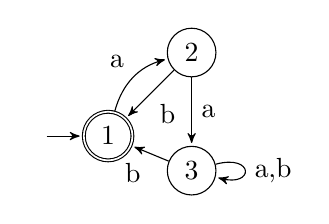
\begin{tikzpicture}[>=stealth',shorten >=1pt,auto,node distance=1.5cm]
                \tikzset{every state/.style={minimum size=0.2cm}}
                    
                    \node[initial,state,accepting]  (a1)      {1};
                    \node[state] (b1)  [above right of=a1]    {2};
                        \node[state] [below of=b1](c1)      {3};
                \path[->]
                        (a1)  edge [bend left] node {a} (b1)
                        (c1)  edge[loop right]  node {a,b} (c1)
                        (b1)  edge  node {a} (c1)
                        (b1)  edge  node {b} (a1)
                        (c1)  edge  node {b} (a1)
                        ;
            \end{tikzpicture}            

            \item	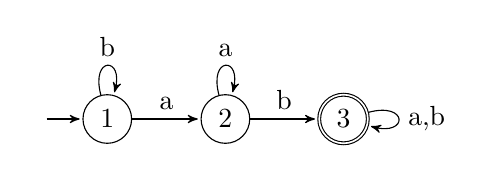
\begin{tikzpicture}[>=stealth',shorten >=1pt,auto,node distance=1.5cm]
                    \tikzset{every state/.style={minimum size=0.2cm}}
                        
                        \node[initial,state]  (a1)      {1};
                        \node[state] (b1)  [right of=a1]    {2};
                            \node[state,accepting] [right of=b1](c1)      {3};
                    \path[->]
                            (a1)  edge  node {a} (b1)
                            (a1)  edge[loop above]  node {b} (a1)
                            (b1)  edge  node {b} (c1)
                            (b1)  edge[loop above]  node {a} (b1)
                            (c1)  edge[loop right]  node {a,b} (c1)
                            ;
            \end{tikzpicture}
            
            \item	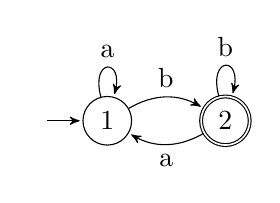
\begin{tikzpicture}[>=stealth',shorten >=1pt,auto,node distance=1.5cm]
                    \tikzset{every state/.style={minimum size=0.2cm}}			
                        \node[initial,state]  (a1)      {1};
                        \node[state,accepting] (b1)  [right of=a1]    {2};
                    \path[->]
                            (a1)  edge[bend left]  node {b} (b1)
                            (a1)  edge[loop above]  node {a} (a1)
                            (b1)  edge[bend left]  node {a} (a1)
                            (b1)  edge[loop above]  node {b} (b1)
                            ;
            \end{tikzpicture}

            \item	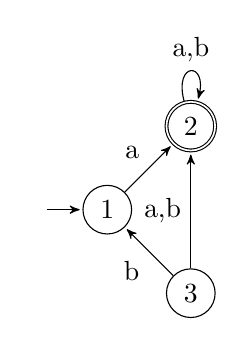
\begin{tikzpicture}[>=stealth',shorten >=1pt,auto,node distance=1.5cm]
                    \tikzset{every state/.style={minimum size=0.2cm}}
                        
                        \node[initial,state]  (a1)      {1};
                        \node[state,accepting] (b1)  [above right of=a1]    {2};
                            \node[state] [below right of=a1](c1)      {3};
                    \path[->]
                            (a1)  edge  node {a} (b1)
                            (b1)  edge[loop above]  node {a,b} (b1)
                            (c1)  edge  node {b} (a1)
                            (c1)  edge  node {a,b} (b1)
                            ;
                    \end{tikzpicture}

        \end{enumerate}

    \end{multicols}

\end{problem}


\medskip\begin{problem}[Are regular expressions regular?]

    Fix a finite alphabet $\Sigma$. Is the language consisting of all regular expressions over $\Sigma$ a regular language?

\end{problem}


\end{document}